\chapter{Background and Related Work}
\label{chap:background-and-related-work}

``Code review is a vital element of any long-lived software development project'' \citep[p. 1037]{10.1145/2884781.2884840}. This well-written description is kept as a central point throughout this project and serves well as a justification for why this research is needed.

Open-source projects are vital to the software ecosystem. A paper discussing lessons learned from writing software used by NASA for missions on Mars found that open-source projects outperformed paid-for solutions in terms of maintenance, code quality and support \citep[p. 44]{NorrisMissionCritical}. This means open-source projects can be critically important and therefore research on improving the tools used by open-source projects brings benefits to more than just the open-source project in question.

%\williamnote{Begin: Importance of code review}

\section{Code Review}

The first description of `software inspection' in M. E. Fagan, 1976, describes how `... all changes must be inspected!' \citep[p. 280]{5387093}. Software inspection is the root of modern code review. Though they have their differences, including inspections being `conceived as formal meetings' \citep[p. 27]{7202946}, the idea of inspecting and reviewing a change for problems remains similar.

While some may be tempted to ``blow it up and start over'' with code review, research has found many benefits to the modern code review system not provided or fully covered by other processes. These benefits include:
\begin{itemize}
    \item Assuring the quality of code \citep[p. 2183]{McIntosh2015} \citep[p. 27]{7202946} \citep[p. 181]{10.1145/3183519.3183525}.
    \item Improving security \citep[p. 181]{10.1145/3183519.3183525}.
    \item Checking for consistency of style and design to pre-existing code \citep[p. 181]{10.1145/3183519.3183525}.
    \item Being a `a knowledge sharing tool' \citep[p. 27]{7202946}.
\end{itemize}

However, several papers have found drawbacks that come with modern code review. These include code review being `expensive' in time and money \citep[p. 27]{7202946}, usefulness dropping off for large changes, how assigning appropriate reviewers is a ``challenge'' with this being worse ``in the case of large projects'' \citep[p. 931]{6606642} and how slow code review `causes process stalls' \citep[p. 28]{7202946}.

%\williamnote{Begin: The importance of speed in code review}

As mentioned above, code review being sometimes slow is a drawback of the modern code review system. Google's documentation on this describes how ``if you are not in the middle of a focused task, you should do a code review shortly after it comes in'' \citep{GoogleCodeReviewSpeed}.

Several papers and the Google documentation from above have discussed the negative consequences of slow code review. This includes:
\begin{itemize}
    \item An ``increase[d] ... risk of software degradation'' \citep[p. 519]{9240657}.
    \item Negative impact on code health \citep{GoogleCodeReviewSpeed}.
    \item Negative impact on the number of patches reviewed \citep[p. 67]{7809488}. \citeauthor{7809488}, \citeyear{7809488} found that a reviewer reviews if the ``benefit of review is higher than the cost''.
    \item Disincentivisation of peripheral developers if the review of their patches is much slower than core developers \citep[p. 8]{10.1145/2652524.2652544}.
\end{itemize}

We previously researched how the speed of code review is affected by ``activity, usage and code quality'' in our CS4040 project \citep[p. 1]{WilliamBrownCS4040}. While we did not find any strong links between the factors investigated to the speed of code review, that project did give us an idea about how to collect the data for this research, especially the Bitergia API. %\rcnote{First mention of biterq. Briefly explain what it is and why it is relevant.}.
It also gave us a good idea of related papers to code review which laid the basis for much of the background and related work detailed here \citep[pp. 2-3]{WilliamBrownCS4040}. Overall our previous work was a good starting point for this research and suggests that it could lead to a method that would indeed help speed up code review.

\section{Automation in Code Review}

Past research has found that tests have a `weak positive relationship' to bugs \citep[p. 112]{6605914}. This means that testing in a software project is important to eliminate bugs, and in turn, makes the code both more stable and reliable. Unless these tests are automatically run for the changes that are proposed, the changes could be merged without ensuring that they pass the tests. If the tests don't pass this won't reduce the number of bugs and is likely to increase the bug count.

In the MediaWiki project both integration and unit tests are used \citepmediawiki{mediawiki:php-unit-testing} as well as automated tools that inspect for issues (such as PHPCodeSniffer \citepmediawiki{mediawiki:php-code-sniffer} and Phan \citepmediawiki{mediawiki:phan}), which are run automatically when changes are uploaded and also before changes are merged \citepmediawiki{mediawiki:continuous-integration}. These tests are run to help ensure that the master branches remain in an (almost) constantly deployable state \citepmediawiki{mediawiki:continuous-integration}.

These automated inspection tools cover the entire code base but are limited in what they can do. While they can see syntax problems \citepmediawiki{mediawiki:php-code-sniffer} and potential security issues \citepmediawiki{mediawiki:phan}, they can't fully understand the meaning or intended meaning of changes to the code.

While integration and unit tests exist for MediaWiki, the coverage of these tests is poor for many repositories (as shown in Figure~\ref{fig:extension-test-coverage-example}) \citepmediawiki{ExtensionTestCoverageMediaWiki}. Research has found that ``the effort for writing tests for existing, untested code is difficult to estimate and might have a negative cost-benefit ratio'' \citep[p. 4]{7107469}. As such, poorly or untested code in MediaWiki may be seen as not worth it or difficult to achieve. Furthermore, the author thinks that volunteer developers and reviewers without the expectation to enforce testing may skip tests when the file is already untested.

\begin{figure}[htb]
    \centering
    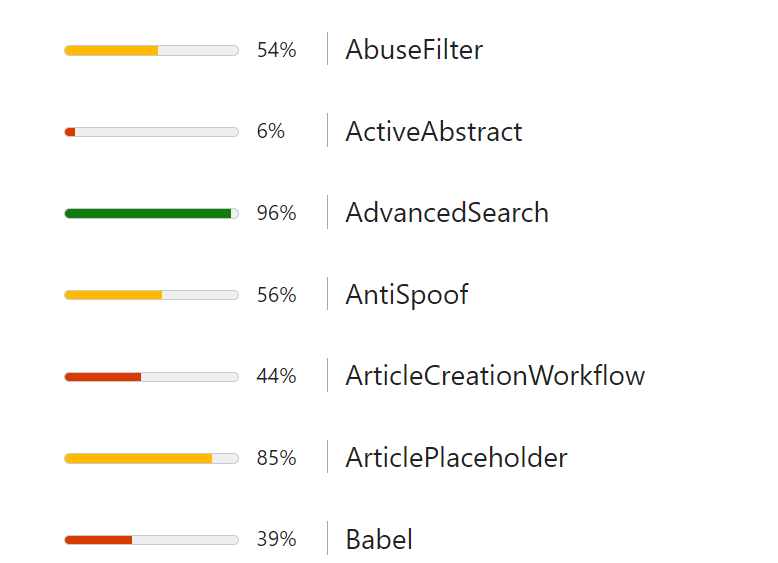
\includegraphics[scale=0.6]{images/MediaWiki-extensions-test-coverage-list.png}
    \caption[Excerpt of test coverage sorted by extension name.]{Excerpt of test coverage sorted by extension name. Image credit: Screenshot of section of the page \url{https://doc.wikimedia.org/cover-extensions/}. Accessed 30 April 2023.}
    \label{fig:extension-test-coverage-example}
\end{figure}

\section{Necessity of Human Review}

Code review, by its very definition, is ``an inspection of a code change by an independent third-party developer'' \citep[p. 141]{7081824}. If a code review system only used a computer to review, there would not be one person responsible for a change as the computer program that approved the change would have been contributed to by many authors. Having a human in the loop before the change is approved would at the very least give a person responsibility for a change.

Some repositories are more sensitive and/or critical than others. This means that the thoroughness of the average review can vary between repositories. In the MediaWiki project, extensions that are deployed on WMF wikis (which includes the English Wikipedia) \citep{wikitech:Deployments/Train} are often subject to more scrutiny such as continuous integration tests that run over all WMF deployed code \citep{github:integration-config-extension-gate}. This is because the changes are deployed every week \citep{wikitech:Deployments/Train}, so there is less time to review changes after their merge. Wikipedia is one of the most visited sites on the web \citep[p. 2365]{10.1145/3366423.3380300} \citep[p. 249]{10.1145/3442381.3450136} and broken changes could cause serious outages or security flaws that affect the millions of visitors.

An example of such a repository is the repository for the CheckUser extension. The extension collects and stores IP Addresses, XFF strings and user agent strings which are connected to registered and unregistered users \citep[p. 158]{10.1145/2030376.2030394} \citep{ExtensionCheckUser}. This extension has been noted in previous research around performing `link spam` as being an important way such abuse is stopped \citep[p. 158]{10.1145/2030376.2030394}.

The need for stringent review in these more sensitive and critical repositories is therefore heightened compared to an average code review process. This only amplifies the risk taken on by the reviewer who is responsible and also, therefore, means more time would usually be needed before a reviewer could be satisfied that a change was good.

Finding an appropriate reviewer for large software projects is a difficult task. For large projects, many developers editing one file is normal which makes simple inspection of the history of the file to find the appropriate reviewer much harder \citep[p. 931]{6606642}.

This all means that an automatic system in today's code review can benefit from both automation and human review. As such, methods to find a human reviewer would help in most modern code review systems where such a method does not already exist.

\section{Related Work\label{section:related-work}}

Several papers have concluded that a reviewer recommender system would help improve the code review system. In \cite{10.1145/2652524.2652544}, where the paper discusses the issues surrounding peripheral developers being disincentivised from contributing patches if core developers have their patches merged much faster, concluded that the delay in feedback could be addressed using a reviewer recommender system \citep[p. 9]{10.1145/2652524.2652544}. Furthermore, in \cite{10.1145/2884781.2884840} that described code review as a ``vital element of any long-lived software development project'' they go on to recommend a reviewer recommender system project for future research and that it ``could be able to help both reviewers and patch writers determine the right person to review a code change at hand'' \citep[p. 1037]{10.1145/2884781.2884840}. The paper goes on to say that there is a large body of research that covers the problem of expertise recommendation but that these solutions do not scale well \citep[p. 1037]{10.1145/2884781.2884840}.

A system exists for the MediaWiki project that named ``ReviewerBot'' uses the Git Reviewers list\footnote{\url{https://www.mediawiki.org/w/index.php?title=Git/Reviewers\&oldid=5899016}. Accessed 3 May 2023} to match users to changes. However, this relies on users adding themselves to this list and this means that the system cannot consider adding new users or users who do not review patches often. The system adds users to changes based on the repository and optionally a path inside the repository, however, only 10\% of people listed used this. This system also does not encourage authors of changes to become reviewers, as it requires the user to know about the list and feel that they are allowed to add themselves as a reviewer to every change. This system also relies on a manually maintained list of users, which brings a cold-start problem for new repositories and could go out of date if inactive users do not remove themselves from the list. An excerpt for this list is shown below in Figure~\ref{fig:checkuser-extension-reviewer-list}.

\begin{figure}[h]
    \centering
    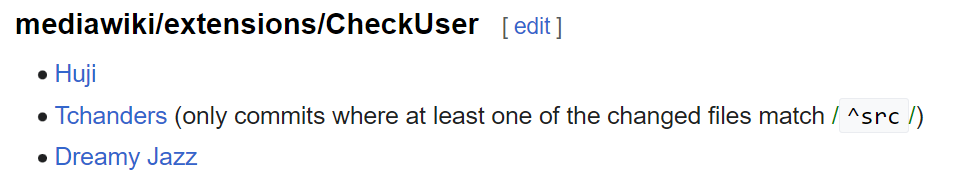
\includegraphics[scale=0.9]{images/git-reviewers-list-checkuser.png}
    \caption[Git reviewers list for the CheckUser extension.]{Git reviewers list for the CheckUser extension. Image credit: Screenshot of the page \url{https://www.mediawiki.org/wiki/Git/Reviewers\#mediawiki/extensions/CheckUser}. Accessed 30 April 2023.}
    \label{fig:checkuser-extension-reviewer-list}
\end{figure}

Back in 2009, a system was implemented over two open-source projects that predicted reviewers for the open-source project Firefox and Mozilla core \citep[p. 1]{jeong2009improving}. This project made implementations to predict whether a patch would be accepted and also implemented a system to predict who reviewed a patch \citep[p. 2]{jeong2009improving}. This system worked on the Bugzilla system, which is a bug-reporting system \citep{bugzilla:about}. To the best of our knowledge, this seems to be one of the first implementations and seems to have been the basis for other research mentioned here.

Research performed by \cite{10.1145/2593702.2593705} was implemented based on a system using file path similarity, where reviewers who had reviewed changes on files with similar paths were recommended for a given change \citep[p. 120]{10.1145/2593702.2593705}. This system was found to work well `in two of the three OSS projects` (Open Source Software).

The authors of the above research later expanded their work making a `file location-based' recommender system which was researched and tested on four different open-source projects \citep[p. 141]{7081824}. Named RevFinder, the system \enquote{accurately recommended 79\% of reviews with a top 10 recommendation} and was deemed as 3 times better than the baseline approach \citep[p. 141]{7081824}. This system was trained on projects that use the Gerrit code review system \citep[p. 142]{7081824} like MediaWiki does \citepmediawiki{mediawiki:gerrit}.

In \cite{7332472} the research compares its implementation against \cite{7081824}, and finds that it \enquote{outperforms REVFINDER by a substantial margin}\footnote{``REVFINDER'' is the implementation built by \cite{7081824}.} \citep[p. 266]{7332472}. It also finds that selecting previous reviews from varying \enquote{number of past days M} in most cases keeps the MRR and Top-k values \enquote{stable for various M values} \citep[p. 268]{7332472}.

Later research by \cite{9240650} expanded on the data-set created by \cite{7081824} and also data from selected GitHub projects \citep[p. 501]{9240650}. This research, which covered more projects, gives \enquote{accuracy over 70\% in the top-10 across all the projects} \citep[p. 507]{9240650}. This research compared its implementation against \cite{7081824} and \cite{7332472}. The research also states that the implemented tool finds 466 plain developers (developers who only write code) who over time become developer-reviewers \citep[p. 507]{9240650}. This research suggests that a tool could encourage non-reviewing developers to make reviews, which could help address the lack of reviewers in a project.

A different system based on different projects was also created by \citeauthor{7328331} and was evaluated against the RevFinder system mentioned above \citep[p. 536]{7328331}. The research found that their implementation performed much better than the RevFinder system \citep[p. 539]{7328331}.

A method used by the company Tencent is described and evaluated in \citeauthor{10.1145/3510457.3513035}, however, this system uses configuration files recording ownership and authorship of
code to recommend \citep[p. 117]{10.1145/3510457.3513035}. This makes it similar to the current Git reviewers list system that is implemented in MediaWiki, though the configuration files are likely to be better maintained. However, this paper does find that other implementations discussed here perform worse on
proprietary projects than open-source projects \citep[p. 120]{10.1145/3510457.3513035}.

One solution aimed at providing a user-friendly automatic recommendation implementation is UnReview \citep{UnReviewIoMedium}. The project was acquired by GitLab in June 2021 \citep{gitlab-acquires-unreview} However, the website for this is now offline and the last published update around this project was from June 2022 \citep{gitlab-unreview-year-later}. The service has gone through a closed beta \citep{gitlab-unreview-year-later}, so the tool does exist but access to this tool is not possible for our research.

A plugin to the Gerrit system exists that adds users as reviewers for the change that authored most of the lines touched by the change \citep{gerrit-git-blame-plugin}. Because this system integrates with Gerrit, it makes it applicable to the MediaWiki project, however, it only performs analysis on users who have authored changes. This can be built on to make a tool that works more generally. This is also not installed in the installation of Gerrit used by the MediaWiki project.

Recommender systems using deep learning have been discussed in \citeauthor{nagy2021review}, and the paper was a useful starting point on how to implement a recommender system using machine learning and specifically neural networks \citep[p. 174]{nagy2021review}.

In \citeauthor{gupta2018intelligent} \citeyear{gupta2018intelligent}, the authors created a tool that uses deep learning to automatically make suggestions on submitted changes. This system was found to have been positively received by the users of the tool \citep[p. 8]{gupta2018intelligent} and was described by the authors as `a flexible, adaptive, and easy-to-configure automatic code review system' \citep[p. 9]{gupta2018intelligent}. This suggests that automation can cover many aspects of a standard code review.

The related work in automation in code review has described implementations or implemented systems that automatically recommend reviewers. However, we could not find any paper that focused on the MediaWiki project. While the work reported in this section may have been tested for other repositories, the previous research suggests that this project should still break new ground.